\documentclass{standalone}
\usepackage{tikz}

\begin{document}
\usetikzlibrary{positioning,shapes,arrows,snakes}
\definecolor{yellowish}{HTML}{FFE699}
\definecolor{grayish}{HTML}{D9D9D9} 
\tikzset{
   rect/.style={
      align=center,
      text=black,    
      minimum width=2.5cm,
      minimum height=2cm}
}
\tikzset{
   done/.style={rect, fill=grayish }
}
\tikzset{
   todo/.style={rect, fill=yellowish}
}
\tikzset{
   arrow/.style={line width=1mm}
}
\centering

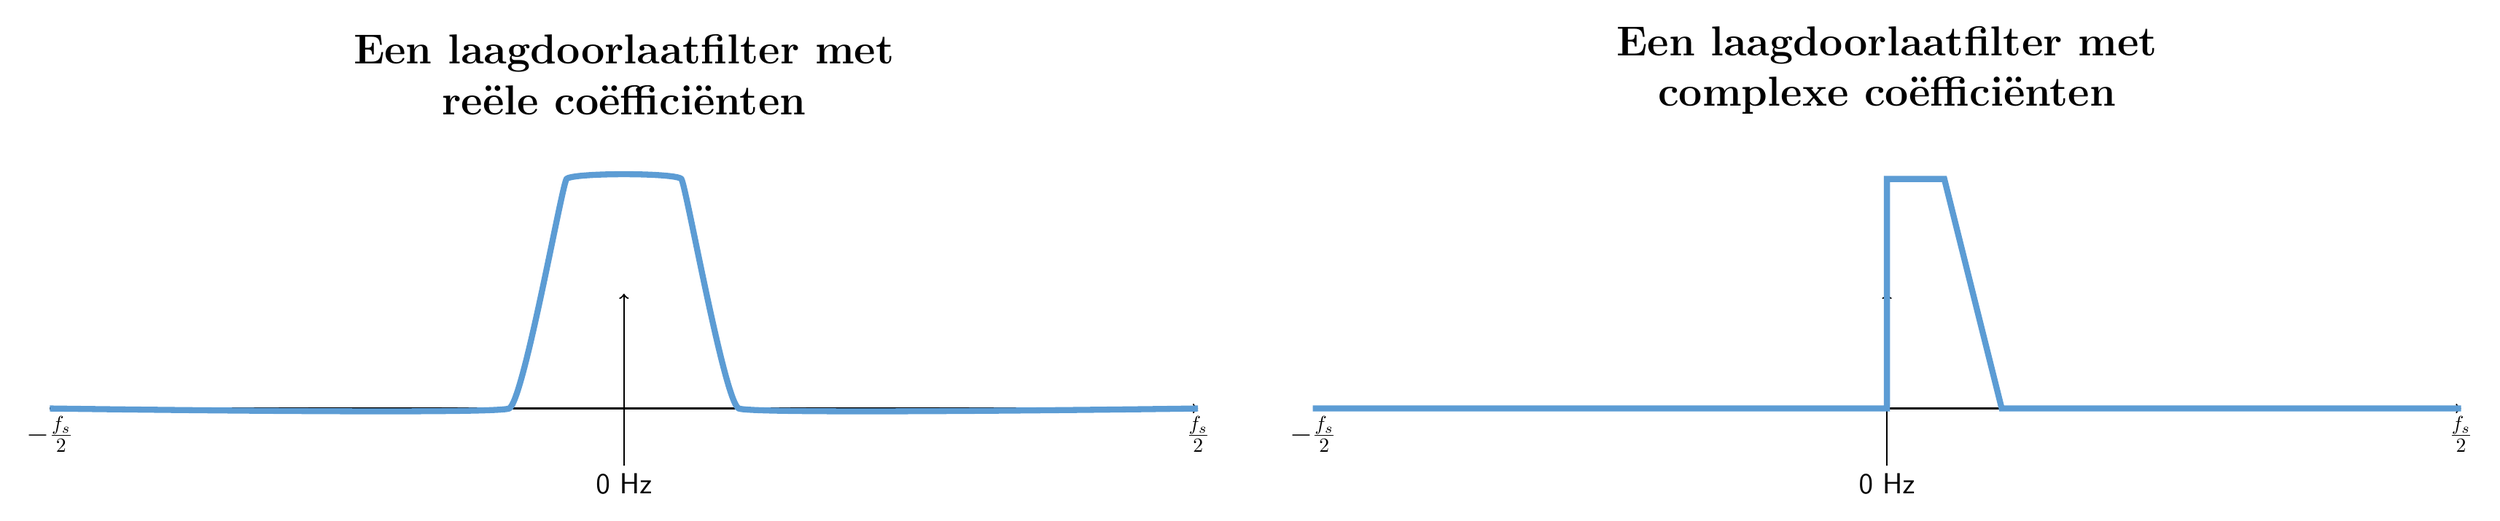
\begin{tikzpicture}[font=\sffamily\Large,scale=2] 
   \definecolor{babyblueeyes}{rgb}{0.36, 0.61, 0.83}   
   \draw[->, thick] (-5,0) node[below]{$-\frac{f_s}{2}$} -- (5,0) node[below]{$\frac{f_s}{2}$};
   \draw[->, thick] (0,-0.5) node[below]{0 Hz} -- (0,1);
   \draw[babyblueeyes, smooth, line width=3pt] plot[tension=0.1] coordinates{(-5,0) (-1,0) (-0.5,2) (0.5,2) (1,0) (5,0)};
   \draw[->,thick] (6,0) node[below]{$-\frac{f_s}{2}$} -- (16,0) node[below]{$\frac{f_s}{2}$};
   \draw[->,thick] (11,-0.5) node[below]{0 Hz} -- (11,1);
   \draw[babyblueeyes, smooth, line width=3pt] plot[tension=0] coordinates{(6,0) (11,0) (11,2) (11.5,2) (12,0) (16,0)};
   \draw[font=\huge\bfseries] (0,2.5) node[above,align=center]{Een laagdoorlaatfilter met\\reële coëfficiënten};
   \draw[font=\huge\bfseries] (11,2.5) node[above,align=center]{Een laagdoorlaatfilter met\\complexe coëfficiënten};
\end{tikzpicture}
\end{document}